\chapter{Deep Search Queries}
\label{ch:findings_chapter}

\section{Introduction}
Sieveable enables users to perform queries across multiple levels to meet diverse search goals.
It can find apps with specific listing fields, UI structures, manifest attributes, and API calls.
Sieveable can produce results beneficial to several stakeholder groups:
a) User interface design researchers can use Sieveable to find apps with specific design structures.
b) Accessibility researchers can use it to find answers to accessibility questions.
c) Privacy and security researchers can use it to find apps that request an unusual number of permissions or use vulnerable APIs.
d) Program analysts can use Sieveable to reduce the time to find examples of interest to apply defect analysis.
e) Data mining researchers can mine applications efficiently and build machine-learning applications at large scale without incurring the overhead of collecting and indexing large datasets.
In previous works \cite{Alharbi_2015_MobileHCI}, these types of analyses would require custom scripts to be written and executed on a cluster, which would require several days of work.
In contrast, Sieveable is able to reduce the problem to a simple search query, which takes an analyst only seconds to specify and minutes to run.

In this section, we present several illustrative search queries to show that Sievable enables users to conduct many types of analyses.

\section{Design Queries}
% we have lots of those
\subsubsection{UI Screen}
In mobile app design, designers and developers tend to create a set of UI screens that serve a common purpose. 
We can use Sieveable to find common screens and search for design alternatives.
We can also aggregate the results and find trends in implementing one design over the other.

\underline{\textbf{Sign In:}}
Many apps allow users to sign into their accounts to enable them to use certain features.
Some apps use the sign in screen as the first screen that welcomes new users to their applications.
Sign in screens usually take the form of a single sign in button.
To find such examples, we query Sieveable for apps that use a Button with the phrase ``Sign In''. 
We can also include the number of downloads in the result fields to reflect on how popular they are:
\begin{minted}{xml}
    MATCH app
    WHERE
        <Button android:text="Sign In"/>
        <downloads>(*)</downloads>
    RETURN app, $1
\end{minted}
This query resulted in 1,459 apps. The first response containing 10 results was received in 1.62 seconds while the request to return all the results completed in 4 minutes. By analyzing the downloads count for the results, we can show the distribution of downloads for all apps that use this design option (Figure~\ref{fig:fig_signInDownloadDist}a).

We can use Sieveable to find alternative ways of designing a sign in screen.
For example, we can also search for apps that use a TextView as a sign in button and obtain their download count to compare it with the previous results:
\begin{minted}{xml}
    MATCH app
    WHERE
        <TextView android:text="Sign In"/>
        <downloads>(*)</downloads>
    RETURN app
\end{minted}
This query returned 577 apps.
We received the first response that contains 10 results in 1.2 seconds while the request to return all the results completed in 1.8 minutes. Figure~\ref{fig:fig_signInDownloadDist}b shows the apps by their downloads amount.

\begin{figure}[ht]
\centering
\subfloat[Sign in Button]{{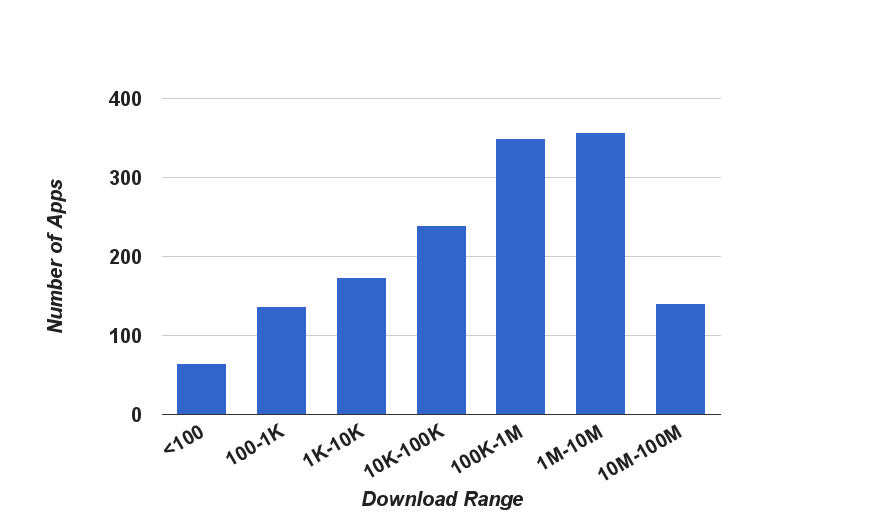
\includegraphics[scale=0.3]{figures/sieveable-deep-search/signInBtnDownloadDist} }}%
\qquad
\subfloat[Sign in TextView]{{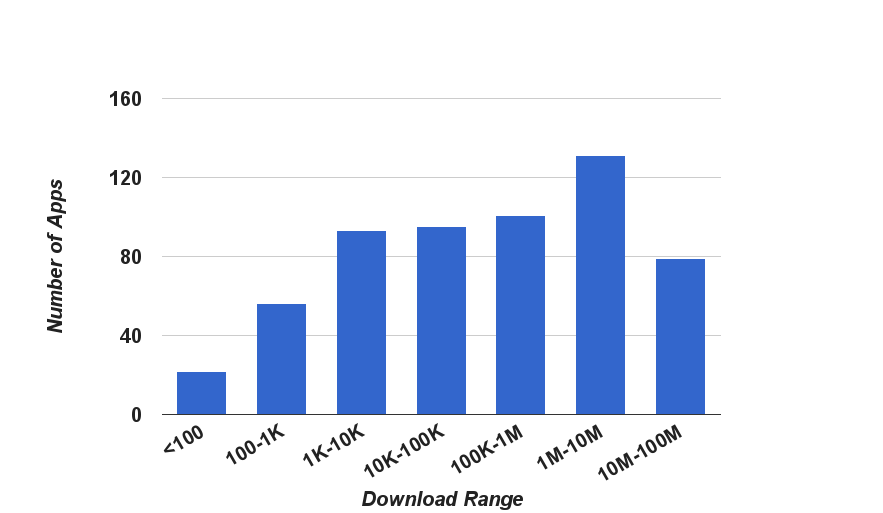
\includegraphics[scale=0.3]{figures/sieveable-deep-search/signInTextViewDownloadDist} }}%
\caption{Download distribution of apps that have a sign in screen.}%
\label{fig:fig_signInDownloadDist}
\end{figure}

\subsubsection{Design Interactions}
Mobile apps feature unique interactions allowing users to navigate within the app using various touch gestures and UI controls. We can use Sieveable to explore real-world examples of apps that use a combination of gestures and UI controls and identify common patterns among them.
	
\underline{\textbf{Pull Down to Refresh:}}
In mobile app design, there is a common UI interaction gesture called ``Pull down to refresh'' \cite{brichter2010user}.
It is used for in-app content updates, allowing users to see new content by scrolling a view vertically.
Some apps use this mechanism to push content updates to the UI view when it is requested by the user as an alternative to auto-updates, which may consume critical mobile device resources such as battery and network.
In Android, this interaction gesture is not built into the standard UI widgets, so developers need to use additional library APIs to implement this gesture.
One commonly used library is the  Android Support Library, which includes a layout view called SwipeRefreshLayout that enables developers to implement this gesture.
In addition to declaring this view in the UI layout file, developers need to register event listeners in the code to respond to the gesture and refresh the content.
We are also interested in finding the top three categories of the apps that use this interaction mechanism.
To find such examples, we can use Sieveable to search for apps by three levels search criteria (UI, code, and listing details).

\begin{minted}{xml}
MATCH app
WHERE
<android.support.v4.widget.SwipeRefreshLayout>
<ListView/>
</android.support.v4.widget.SwipeRefreshLayout>
<code 
class=
"android.support.v4.widget.SwipeRefreshLayout"
method="setOnRefreshListener" />
<store-category>(*)</stroe-category>
RETURN app, $1
\end{minted}

This query produced 277 apps.
The first 10 results response was received in 1.7 seconds while the request to return all the results completed in 49 seconds.
The query results include the list of store categories for these apps. We found that the top categories for apps that use the the pull to refresh gesture are: Sports (14\%), News \& Magazines (8.9\%), and Social (8.9\%).
This highlights the amount of updatable content offered by apps in these categories.

\section{Security Queries}
The popularity of mobile apps have increased the exploitation of their vulnerabilities.
Security researchers and mobile apps security analysts use sophisticated techniques to detect software vulnerabilities.
However, their techniques are largely constrained by the availability of samples of apps that are vulnerable to attacks.
Sieveable can be used to perform code search queries for apps that are vulnerable to attacks as a result of weak API implementations.
The search query can be combined with multiple search criteria to restrict the search to specific API versions.

\underline{\textbf{WebView:}}
A webView is a UI component that displays web pages. 
This component is widely used in mobile apps to display web pages or display banner ads.
While the webView is a great feature that helps developers deliver rich content to their users, it can also become the most dangerous component in an app.
For example, developers can enable JavaScript in a webView and expose the Java object's methods to the JavaScript interface.
This allows untrusted  content viewed in the webView to use reflection to access all public and inherited methods like \textit{Class.forName("java.lang.Runtime")}.
An attacker may send a link to the user of a vulnerable app and gain access to all device resources or wipe the entire device content. 
This vulnerability was fixed in Android 4.2 but the fix is not effective unless the app targets the API level 17 or higher \cite{WebViewVulnerability}.
Sieveable can be used to find apps that are possible candidates for this vulnerability.
We can search for apps that set the Manifest attribute \textit{targetSdkVersion} to a value less than 17.  Below is an example query.

\begin{minted}{xml}
	MATCH app
	WHERE
	<code 
	class="android.webkit.WebView" 
	method="addJavascriptInterface" />
	<uses-sdk android:targetSdkVersion="12" />
	RETURN app
\end{minted}

This query resulted in 66 apps. The first 10 results returned in 2.5 seconds and the entire request completed in 17 seconds.

\underline{\textbf{Permissions:}}
The security permissions system is the core component of Android security.
Apps have no access to any sensitive operations, hardware resources, or user's data without explicitly asking for permissions. These permissions are granted at install time by the user.
Apps may also declare custom permissions to protect access to certain app features.
To distinguish between custom app permissions and system permissions, the name of system permissions start with "android.permission.*"
Malicious apps tend to request an unusual number of permissions with more frequently on SMS-related permissions \cite{zhou_2012_SP_dissecting}.
We can use Sieveable to find apps that request a large number of system permissions.
For example, we can use the following query to find apps that request 11 or more system permissions and at least an SMS related permission.

\begin{minted}{xml}
	MATCH app
	WHERE
	<uses-permission 
	android:name= "android.permission.*" 
	__min="11" />
	<uses-permission 
	android:name= "*_SMS" />
	RETURN app
\end{minted}

This query produced 5,708 apps in 1.4 minutes. The first 10 results were received in 122 milliseconds.
\section{Program Analysis Queries}
Static program analysis tools are used to examine the source code statically to detect vulnerabilities and possible runtime errors.
Perhaps the most common approach applied in static analysis is searching plain text source files for lines matching a string.
Opening a large number of files, scanning them for matches and combing the results with other parsing tools (e.g., UI and Manifest) is a frustrating process. 
In addition, finding a sample of apps that match a given criteria (e.g., permissions, UI structure) along with the source code text search is a challenging search task.
Static analysis researchers are still constrained by the lack of a large-scale comprehensive search systems to work with.
Sieveable's complete view of the app helps researchers find samples by multiple search criteria and focus their efforts on designing more rigorous static analysis tools.
This is in particular valuable for static analysis tools because it reduces the overhead of obtaining samples and increases the sample size.

\underline{\textbf{Overprivilege Analysis:}}
In Android, application developers may require a number of permissions in the AndroidManifest file without actually using permission protected API calls. Such apps are considered overprivileged. 
Researchers have developed tools that perform overprivilege analysis on apps' source code \cite{felt2011android,au2012pscout}.
These tools work on the decompiled code by constructing a call graph over the entire app and performing traversal to identify API calls that are unreachable.
Their tools could be scaled by using our search system. 
Sieveable can be used to find apps that request a particular permission and declare permission protected API calls.
Static tools can be used to analyze the results to determine whether these API calls are unreachable.
For example, below is a query that searches for apps that request the \textit{Camera} permission and declare the \texttt{android.hardware.Camera open()} API method.

\begin{minted}{xml}
	MATCH app
	WHERE
	<code class="android.hardware.Camera"
	method="open"/>
	<uses-permission 
	android:name="android.permission.CAMERA"/>
	RETURN app
\end{minted}

This query resulted in 9,846 apps. The first 10 results were received in 25 seconds, while the entire query took 36.4 seconds to complete.

% Bug Fixes
\underline{\textbf{{Bug Fixes:}}}
Mobile apps are updated regularly to improve stability and fix bugs.
Updates that include bug fixes are especially interesting to bug finding tool builders.
Android allows developers to list the log of changes for the recent app update in a listing details section named ``What's New''.
This information might be valuable to a program analyst who is interested in understanding various attempts to fix bugs and evaluating them.
We can use Sieveable to find apps with potential bug fixes to common developer errors.
For example, Android uses the Service API for running long operations in the background.
However, the Service API might be confusing to new developers since the Service is not necessarily running in a background thread.
Instead, it runs in the app's main thread by default which causes the app to crash in ``Application Not Responding'' (ANR) error.
We can use Sieveable to get a set of apps that might be candidates for bug fixes related to the use of background services. The query below searches for apps that use the Service API and mention the phrase ``bug fixes'' in the ``What's new'' listing details field.

\begin{minted}{xml}
	MATCH app
	WHERE
	<code class="android.app.Service"
	method="onStartCommand"/>
	<whats-new>bug fixes</whats-new> 
	RETURN app
\end{minted}

This query returned 2,119 apps in 16 seconds. The first 10 results were received in 70 milliseconds.

